\chapter{Il Progetto ARES}
\section{Presentazione del videogioco ARES}
Il progetto ARES consiste nello sviluppo di un videogioco appartenente al genere \textit{First-Person Shooter} (FPS), progettato per una distribuzione multipiattaforma su sistemi operativi macOS e Microsoft Windows. L'opera si prefigge l'obiettivo di raggiungere standard qualitativi paragonabili alle produzioni di fascia "AAA", puntando su un'elevata fedeltà visiva e su un'immersività garantita da scenari complessi e dettagliati.

Dal punto di vista tecnico, il software è stato realizzato utilizzando il motore grafico Unity, avvalendosi specificamente della \textit{High Definition Rendering Pipeline} (HDRP). Questa scelta è stata dettata dalla necessità di gestire sistemi di illuminazione avanzata di tipo \textit{Mixed} (combinazione di luci in tempo reale e pre-calcolate) e materiali ad alta risoluzione, fondamentali per caratterizzare le diverse ambientazioni di gioco, che spaziano da complessi industriali a quartieri urbani densamente popolati.

\begin{figure}[htbp]
    \centering
    \begin{minipage}{0.48\textwidth}
        \centering
        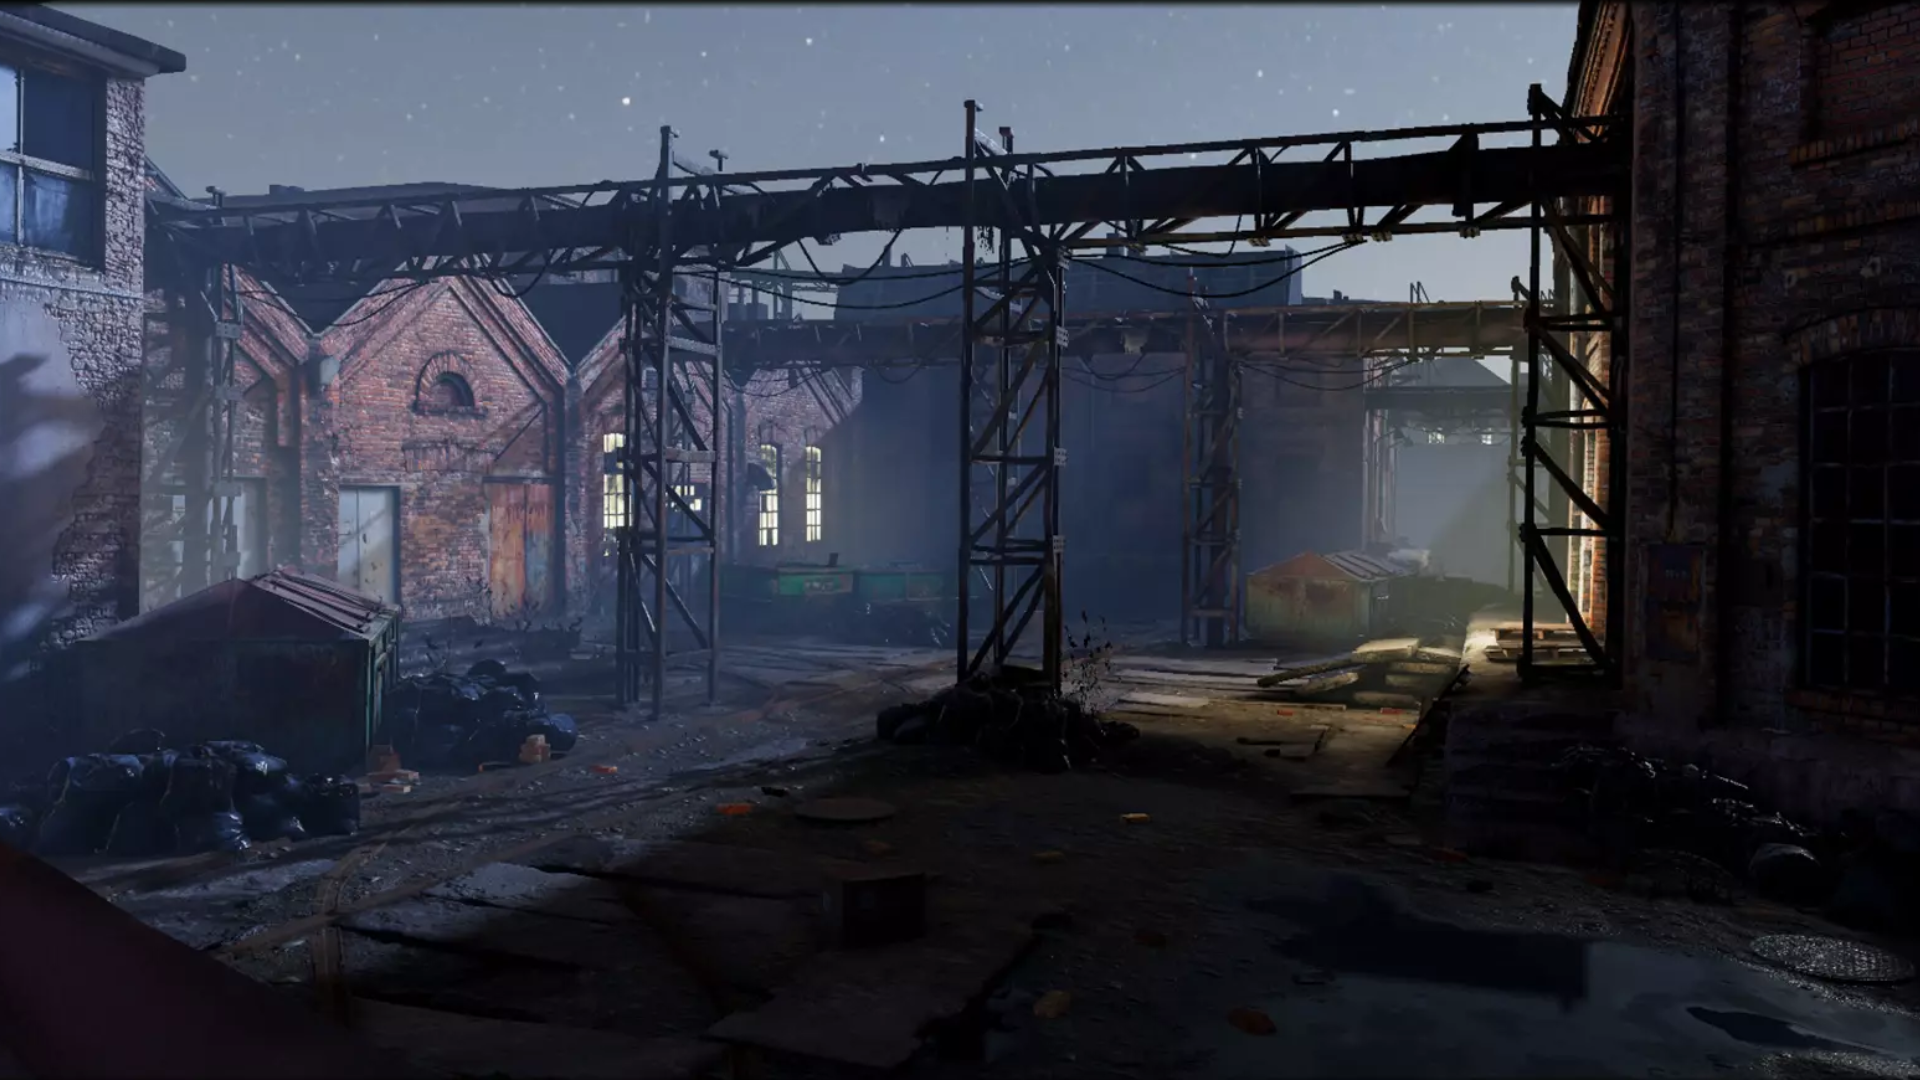
\includegraphics[width=\textwidth]{immagini/map_urban.png}
    \end{minipage}
    \hfill % Spazio flessibile tra le due immagini
    \begin{minipage}{0.48\textwidth}
        \centering
        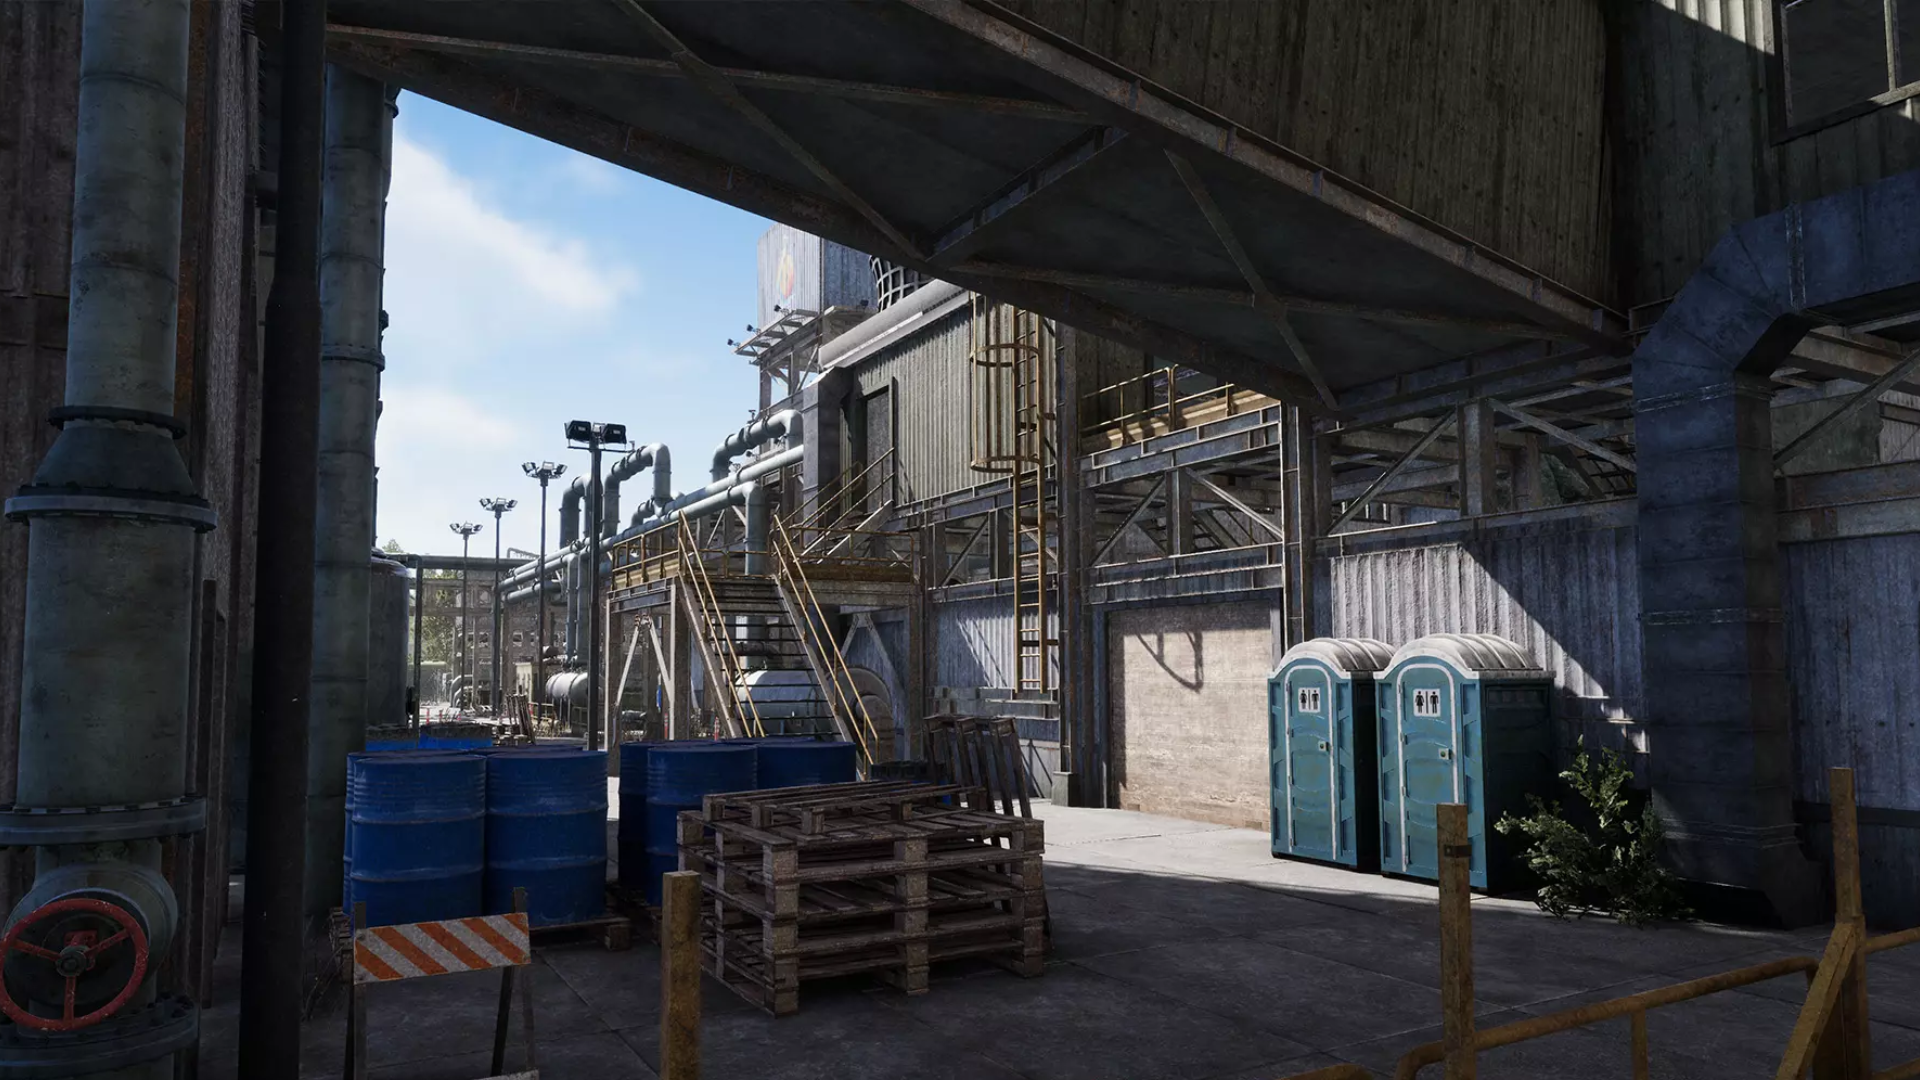
\includegraphics[width=\textwidth]{immagini/map_chemical.png}
    \end{minipage}
    
\end{figure}

Attualmente, il progetto si presenta in una fase di sviluppo avanzata e funzionalmente completa: le meccaniche di base del \textit{gameplay} risultano interamente implementate e il titolo è pienamente giocabile. Nonostante le prestazioni rilevate sulla piattaforma di test (Apple M2 Pro) si attestino su valori ottimali di circa 60 FPS con impostazioni grafiche massime, la vastità delle mappe e l'elevato numero di vertici da renderizzare pongono sfide significative per l'hardware meno performante.

Lo stage si inserisce dunque in questa fase critica del ciclo di vita del software, con l'obiettivo di rifinire la gestione delle risorse grafiche e preparare il motore di gioco per l'introduzione dei contenuti finali e il successivo rilascio. 

Maggiori informazioni sono reperibili presso il sito ufficiale: \\ \url{https://aresofficial.net}.

\section{Motivazioni e obiettivi}
L'attuale mercato dei videogiochi \textit{First-Person Shooter} risulta estremamente competitivo e caratterizzato da standard tecnici elevatissimi. In questo scenario, il progetto ARES nasce con una forte impronta strategica rivolta all'ecosistema macOS, una piattaforma storicamente meno presidiata dai titoli FPS di fascia alta, con l'intento di offrire agli utenti Apple un'esperienza di gioco di qualità comparabile alle produzioni Windows.

Tuttavia, l'obiettivo centrale del presente lavoro di tesi trascende la specifica piattaforma di riferimento, focalizzandosi sull'ottimizzazione trasversale delle prestazioni grafiche su tutti i sistemi operativi supportati. Indipendentemente dall'hardware utilizzato, la fluidità di gioco rappresenta il fattore critico per garantire un'esperienza utente soddisfacente in un titolo competitivo. La ricerca si pone dunque il compito di individuare un \textit{trade-off} ottimale tra fedeltà visiva e velocità di calcolo, massimizzando l'efficienza della pipeline di rendering HDRP per garantire stabilità e alte prestazioni su un'ampia gamma di configurazioni hardware.

Nello specifico, si prefiggono i seguenti obiettivi tecnici e formativi:
\begin{itemize}
\item \textbf{Analisi delle prestazioni:} utilizzo avanzato dello \textit{Unity Profiler} per identificare i \textit{bottleneck} del sistema e comprendere l'impatto dei processi sulla GPU e sulla CPU.
\item \textbf{Ottimizzazione degli Shader:} revisione degli shader esistenti e sviluppo di nuove soluzioni \textit{custom} per ridurre il carico computazionale senza sacrificare il dettaglio grafico.
\item \textbf{Efficienza geometrica:} studio di tecniche per sostituire, ove possibile, istanze di oggetti 3D complessi con shader specifici, riducendo drasticamente il numero di poligoni e di \textit{draw call} inviate al processore grafico.
\item \textbf{Stabilità del Frame Rate:} garantire che l'ottimizzazione porti non solo a un incremento degli FPS medi, ma soprattutto a una stabilità costante del flusso video per evitare fenomeni di \textit{stuttering} durante le sessioni di gioco più concitate.
\end{itemize}